\begin{figure}[h]
\centering
\begin{tikzpicture}
  \node (circ) {
    \begin{tikzpicture}
      \node[inner sep=0pt] (circuit) {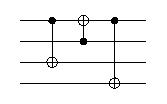
\includegraphics[scale=2, trim={2.5mm 0 2.5mm 0}, clip]{Figures/circuits/interchangeChallenge1}};  
      \node[left=-7mm of circuit.west, rectangle,fill=white,minimum height=22mm, minimum width=8mm] {};
      \node[right=-7mm of circuit.east, rectangle,fill=white,minimum height=22mm, minimum width=8mm] {};
      \node[above left=8mm and -7mm of circuit.west, opacity=0.9] {\footnotesize \(A\)};
      \node[above left=1mm and -7mm of circuit.west, opacity=0.9] {\footnotesize \(B\)};
      \node[below left=1mm and -7mm of circuit.west, opacity=0.9] {\footnotesize \(C\)};
      \node[below left=8mm and -7mm of circuit.west, opacity=0.9] {\footnotesize \(D\)};
      \coordinate[above left=7.2mm and -6mm of circuit.west] (leftPoint);
      \coordinate[above right=7.2mm and -6mm of circuit.east] (rightPoint);
      \pic (cut) {cut=leftPoint/rightPoint};
      \node[right=8.1mm of circuit.west, opacity=0.9] {\footnotesize \(\alpha\)};
      \node[above right=9.8mm and 18.7mm of circuit.west, opacity=0.9] {\footnotesize \(\beta\)};
      \node[right=29.5mm of circuit.west, opacity=0.9] {\footnotesize \(\gamma\)};
      \node[right=-3mm of circuit.north west, font=\itshape] (text) {a)};
    \end{tikzpicture}
  };
  \node[below=5mm of circ] (interchanged) {
    \begin{tikzpicture}
      \node[inner sep=0pt] (circuit) {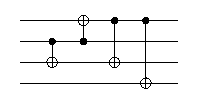
\includegraphics[scale=2, trim={2.5mm 0 2.5mm 0}, clip]{Figures/circuits/interchangeChallenge2}};  
      \node[left=-7mm of circuit.west, rectangle,fill=white,minimum height=22mm, minimum width=8mm] {};
      \node[right=-7mm of circuit.east, rectangle,fill=white,minimum height=22mm, minimum width=8mm] {};
      \node[right=-3mm of circuit.north west, font=\itshape] (text) {c)};
      \node[above left=8mm and -7mm of circuit.west, opacity=0.9] {\footnotesize \(A\)};
      \node[above left=1mm and -7mm of circuit.west, opacity=0.9] {\footnotesize \(B\)};
      \node[below left=1mm and -7mm of circuit.west, opacity=0.9] {\footnotesize \(C\)};
      \node[below left=8mm and -7mm of circuit.west, opacity=0.9] {\footnotesize \(D\)};
      \coordinate[above left=7.2mm and -6mm of circuit.west] (leftPoint);
      \coordinate[above right=7.2mm and -6mm of circuit.east] (rightPoint);
      \pic (cut) {cut=leftPoint/rightPoint};
      \node[right=29.5mm of circuit.west, opacity=0.9] {\footnotesize \(\alpha\)};
      \node[above right=9.8mm and 18.7mm of circuit.west, opacity=0.9] {\footnotesize \(\beta\)};
      \node[right=40.5mm of circuit.west, opacity=0.9] {\footnotesize \(\gamma\)};
      \node[right=8.1mm of circuit.west, opacity=0.9] {\footnotesize \(\chi\)};
      \node[right=-3mm of circuit.north west, font=\itshape] (text) {c)};
    \end{tikzpicture}
  };
  \node[above right=-38mm and 15mm of circ] (hypergraph) {
    \begin{tikzpicture}
      \coordinate (B) at (45:15mm);
      \coordinate (A) at (135:15mm);
      \coordinate (C) at (225:15mm);
      \coordinate (D) at (0,0);
      \draw (A) -- (C);
      \draw (A) -- (B);
      \draw (A) -- (D);
      \node[circle, right=-2.5mm of A, fill=white, inner sep=0pt, minimum size=5mm] {\(A\)};
      \node[circle, right=-2.5mm of B, fill=white, inner sep=0pt, minimum size=5mm] {\(B\)};
      \node[circle, right=-2.5mm of C, fill=white, inner sep=0pt, minimum size=5mm] {\(C\)};
      \node[circle, right=-2.5mm of D, fill=white, inner sep=0pt, minimum size=5mm] {\(D\)};
      \coordinate (leftPoint) at (195:15mm);
      \coordinate (rightPoint) at (75:15mm);
      \pic (cut) {cut=leftPoint/rightPoint};
      \node[above left=5mm and 9mm of A, font=\itshape] (text) {b)};
    \end{tikzpicture}
  };
  \node[below=8.5mm of hypergraph] (hypergraph2) {
    \begin{tikzpicture}
      \coordinate (B) at (45:15mm);
      \coordinate (A) at (135:15mm);
      \coordinate (C) at (225:15mm);
      \coordinate (D) at (0,0);
      \coordinate (aux) at (180:6.5mm);
      \draw (A) -- (B);
      \draw (B) to [bend left] (C);
      \draw (aux) -- (A);
      \draw (aux) -- (C);
      \draw (aux) -- (D);
      \node[circle, right=-2.5mm of A, fill=white, inner sep=0pt, minimum size=5mm] {\(A\)};
      \node[circle, right=-2.5mm of B, fill=white, inner sep=0pt, minimum size=5mm] {\(B\)};
      \node[circle, right=-2.5mm of C, fill=white, inner sep=0pt, minimum size=5mm] {\(C\)};
      \node[circle, right=-2.5mm of D, fill=white, inner sep=0pt, minimum size=5mm] {\(D\)};
      \coordinate (leftPoint) at (195:15mm);
      \coordinate (rightPoint) at (75:15mm);
      \pic (cut) {cut=leftPoint/rightPoint};
      \node[above left=5mm and 9mm of A, font=\itshape] (text) {d)};
    \end{tikzpicture}
  };
\end{tikzpicture}
\vspace*{5mm}
\caption{Example of a circuit \textit{a)} where interchanging CNOTs \(\alpha\) and \(\beta\) saves an ebit. The byproduct gate \(\chi\) in circuit \textit{c)} will be implemented locally, so its addition has no impact. CNOTs \(\alpha\) and \(\gamma\) can be implemented using a single ebit after the interchange. Hypergraph \textit{b)} corresponds to the circuit \textit{a)}. Hypergraph \textit{d)} corresponds to \textit{c)}, and it has one less cut.}
\label{fig:interchangeChallenge}
\end{figure}